\documentclass[12pt, titlepage]{article}
\usepackage{graphicx} 
\usepackage{booktabs}
\usepackage{tabularx}
\usepackage{hyperref}
\hypersetup{
    colorlinks,
    citecolor=black,
    filecolor=black,
    linkcolor=red,
    urlcolor=blue
}
\usepackage[round]{natbib}



\begin{document}

\title{Verification and Validation Report: Truss Tool} 
\author{Maryam Valian}
\date{\today}
	
\maketitle

\pagenumbering{roman}

\section{Revision History}

\begin{tabularx}{\textwidth}{p{3cm}p{2cm}X}
\toprule {\bf Date} & {\bf Version} & {\bf Notes}\\
\midrule
15/04/2023 & 1.0 & Draft version\\
18/04/2023 & 1.1 & Update report\\
19/04/2023 & 1.2 & Update figures and tables\\
\bottomrule
\end{tabularx}

~\newpage

\section{Symbols, Abbreviations and Acronyms}

\renewcommand{\arraystretch}{1.2}
\begin{tabular}{l l} 
  \toprule		
  \textbf{symbol} & \textbf{description}\\
  \midrule 
  T & Test\\
  \bottomrule
\end{tabular}\\

For more detailed Table of Symbols please see \href{https://github.com/Maryamvalian/project741/blob/cfe06182f41c842e3b44aa0eb33d661cf8a3ce79/docs/SRS/SRS.pdf}{SRS}
\newpage

\tableofcontents

\listoftables %if appropriate

\listoffigures %if appropriate

\newpage

\pagenumbering{arabic}

This document is a report on the results of a testing plan for Truss Tool.
Detailed descriptions of the tests can be found in \href{https://github.com/Maryamvalian/project741/blob/cfe06182f41c842e3b44aa0eb33d661cf8a3ce79/docs/VnVPlan/VnVPlan.pdf}{VnV Plan}

\section{Functional Requirements Evaluation} \label{sec_f}

All functional requirements have been met.

\section{Nonfunctional Requirements Evaluation} \label{sec_nonf}

\subsection{Reliability}
The outputs generated by Truss Tool were compared to the \href{https://valdivia.staff.jade-hs.de/fachwerk_en.html}{Existing software} with the same input data. The results were the same and the mean error between the expected value and generated value was less than 0.1.
		
\subsection{Portability}

Truss Tool runs successfully on Windows. The test was done manually.
	
\section{Comparison to Existing Implementation}	

The outputs generated by Truss Tool were compared to the \href{https://valdivia.staff.jade-hs.de/fachwerk_en.html}{Existing software}. the comparison was based on measuring mean error.

\section{Unit Testing}
The detail of the unit tests can be found in VnV Plan section. There were 12 Tests designed and all test cases are performed by test classes built with the help of Pytest. All tests succeed.

\section{Changes Due to Testing}
For the first time running the output test failed. The results didn't completely match the expected value. For some of the members, the results were correct and for some others not. We found the bug in the code was that we did not consider that the force vector's direction is different in two end joints of a member. Figure \ref{Fig_bug} shows the difference. So at the first implementation, we assumed that for each member the direction of force is fixed. After code inspection and debugging, we changed the code to consider a different direction for the member force based on that for which joint we are writing the equations.  

\begin{figure}[h!]
\begin{center}
 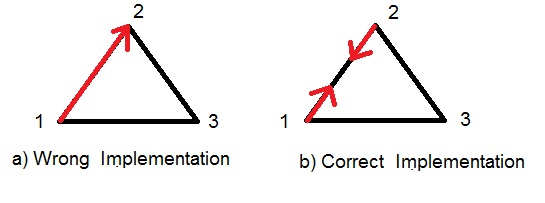
\includegraphics[width=0.7\textwidth]{bug.jpg}
\caption{Changes Due To Testing}
\label{Fig_bug} 
\end{center}
\end{figure}
\section{Automated Testing}
Tools used for automated testing are mentioned in VnV Plan section 4.5. All automated tests were passed successfully.		
\section{Trace to Requirements}
We provide traceability matrices to make it easy for referencing 
what has to be additionally modified if a certain component is changed.
Table  \ref{Table_req} shows the dependencies between the test cases and the requirements.
\begin{table}[h!]
	\centering
	\begin{tabular}{l l} 
		\toprule		
		\textbf{Requirements} & \textbf{Test section}\\
		\midrule 
		R1 & section \ref{sec_f}\\
		R2 & section \ref{sec_f}\\
		R3 & section \ref{sec_f}\\
		R4 & section \ref{sec_f} \\
		NFR1 & section \ref{sec_nonf}\\
		NFR2 & section \ref{sec_nonf}\\
		
		\bottomrule
	\end{tabular}\\
	
	\caption{Traceability Between Test Cases and Requirements} 
	\label{Table_req}
\end{table}
	
\section{Trace to Modules}		
The traceability between test cases and modules are provided in section 6.4 of \href{https://github.com/Maryamvalian/project741/blob/cfe06182f41c842e3b44aa0eb33d661cf8a3ce79/docs/VnVPlan/VnVPlan.pdf}{VnV Plan} 
\section{Code Coverage Metrics}
Not Applicable.
\bibliographystyle{plainnat}
\bibliography{../../refs/References}

\newpage{}


\end{document}